\begin{frame}{Highly Modified Crater}

\begin{figure}
\centering

\begin{subfigure}{0.48\textwidth}
    \centering
    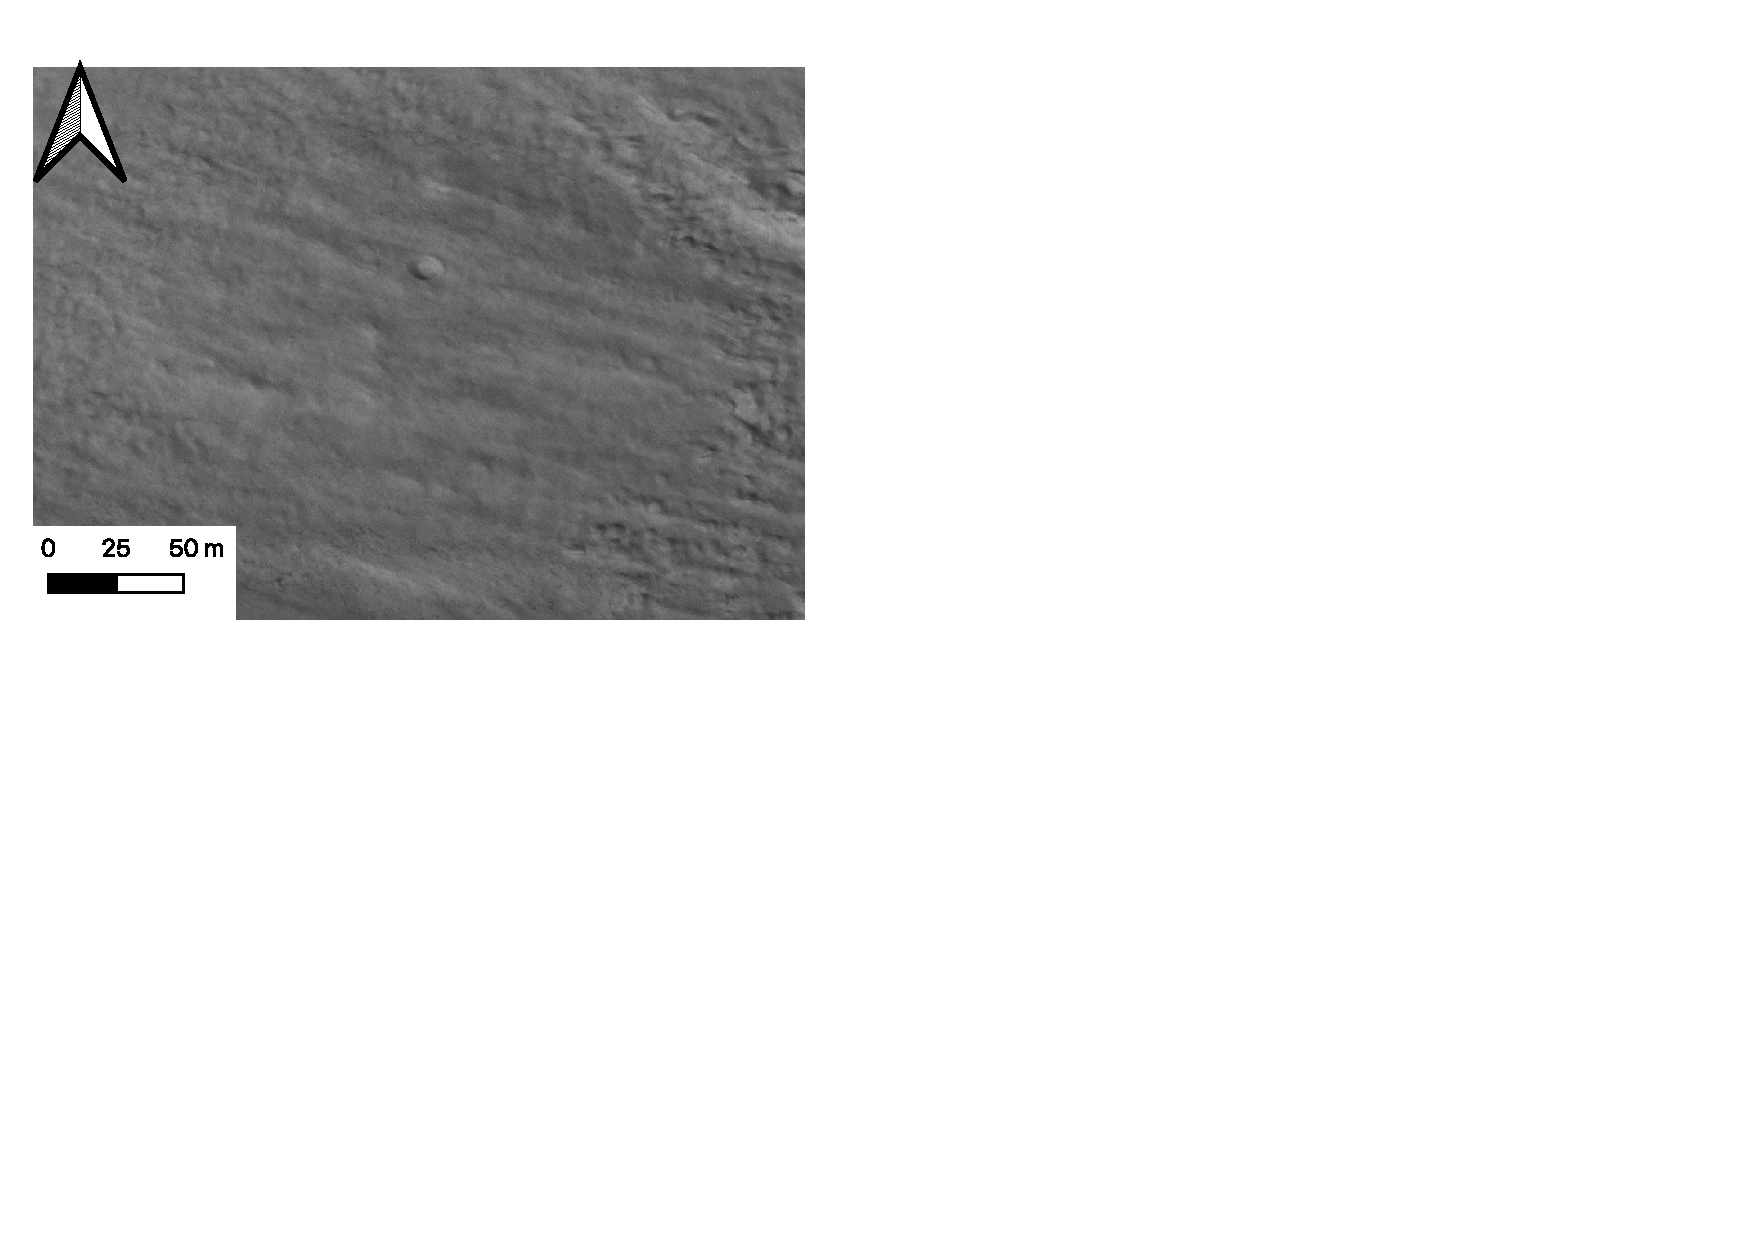
\includegraphics[
        width=\linewidth,
        height=0.65\textheight,
        keepaspectratio
    ]{Figures/HiRISE/GhostCrater_Img.pdf}
    \label{fig:GhostCrater_a}
\end{subfigure}
\hfill
\begin{subfigure}{0.48\textwidth}
    \centering
    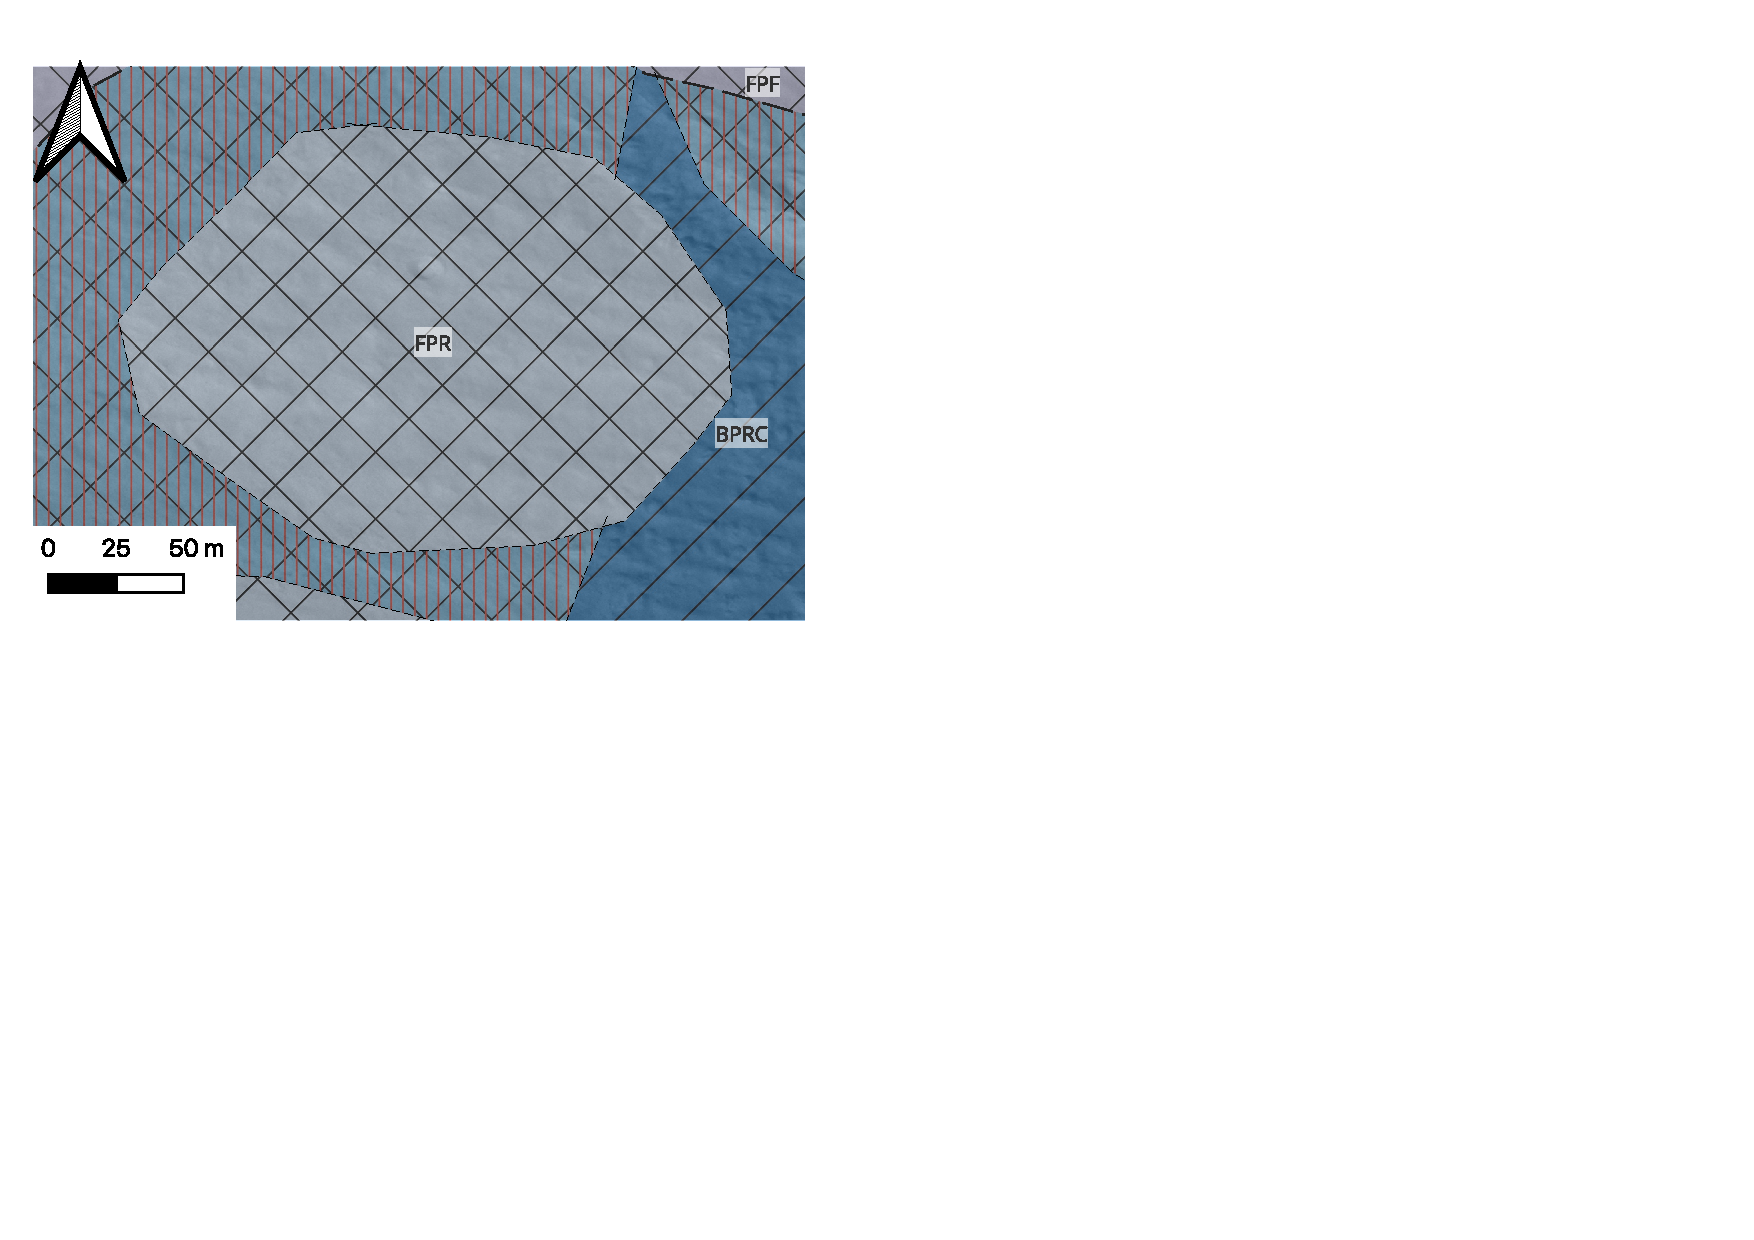
\includegraphics[
        width=\linewidth,
        height=0.65\textheight,
        keepaspectratio
    ]{Figures/HiRISE/GhostCrater_Map.pdf}
    \label{fig:GhostCrater_b}
\end{subfigure}

\caption{Circular smooth surface, suggestive of a ghost crater (centred at $34.62873^{\circ}$N, $16.83217^{\circ}$E).}
\label{fig:GhostCrater}

\end{figure}

\end{frame}
